\documentclass{article}
\usepackage{graphicx}
\graphicspath{{images/}}
\usepackage{hyperref}

\title{TP 4A - Génie Logiciel
Programme Java intégrant modélisation UML, versionning (git)
et tests unitaires (Junit)
}
\author{Mathis Vaugeois - Tanguy Moriceau -  Faustine Guillou}
\date{January 2023}

\begin{document}

\maketitle
\tableofcontents

\newpage
\section{Introduction}

\subsection{Context}
résumé pdf
\subsection{Git}
explication installation github(mathis)
\newpage
\section{Cahier des charges}

\begin{figure}
    \centering
    \includegraphics[width=0.75\textwidth]{diagrammeClasse}
    \caption{Diagramme de Classe.}
    \label{fig:mesh1}
\end{figure}

%\begin{figure}
   % \centering
    %\includegraphics[width=0.75\textwidth]{diagrammeSeq}
    %\caption{Diagramme de Séquence.}
    %\label{fig:mesh2}
%\end{figure}

%\begin{figure}
   % \centering
    %\includegraphics[width=0.75\textwidth]{diagrammeObj}
    %\caption{Diagramme d'Objet.}
    %\label{fig:mesh3}
%\end{figure}

1.Pour réaliser le diagramme de Clase, nous avons d'abord travaillé sur feuille et nous l'avons mis au prope en utilisant InkScape.  \ref{fig:mesh1}. Vous pouvez retrouver ce diagramme sur la page \pageref{fig:mesh1}.
\newline
\newpage
\section{Code de départ}
Après avoir ouvert le projet, nous avons récupéré les commandes données dans le README, cependant cela ne fonctionnait pas.
%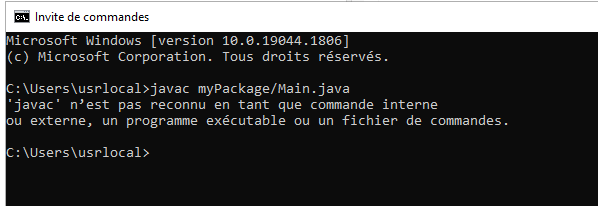
\includegraphics{erreurjavac}
 Le problème est que javac n'était pas reconnu en commande interne. Pour résoudre ce problème, nous avons ajouté javac au PATH.

expliquer cmd (faustine)
\newpage
\section{Développement}
\subsection{Exo 3t}
tanguy
\subsection{Exo4}
\newpage
\section*{Référence}
\url{https://github.com/mathisvaugeois/TPBank-GenieLogiciel}

\end{document}